\begin{figure*}[hbtp]
  \centering
  \subfigure[Overall result]{
    \label{fig:8020-runtime--mean}
    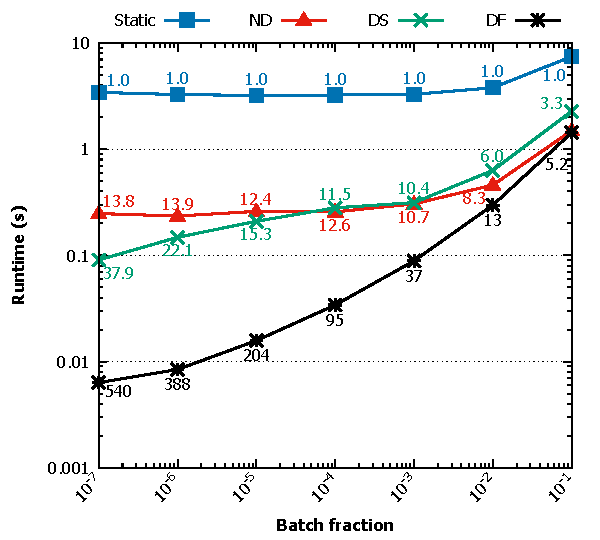
\includegraphics[width=0.38\linewidth]{out/8020-runtime-mean.pdf}
  }
  \subfigure[Results on each graph]{
    \label{fig:8020-runtime--all}
    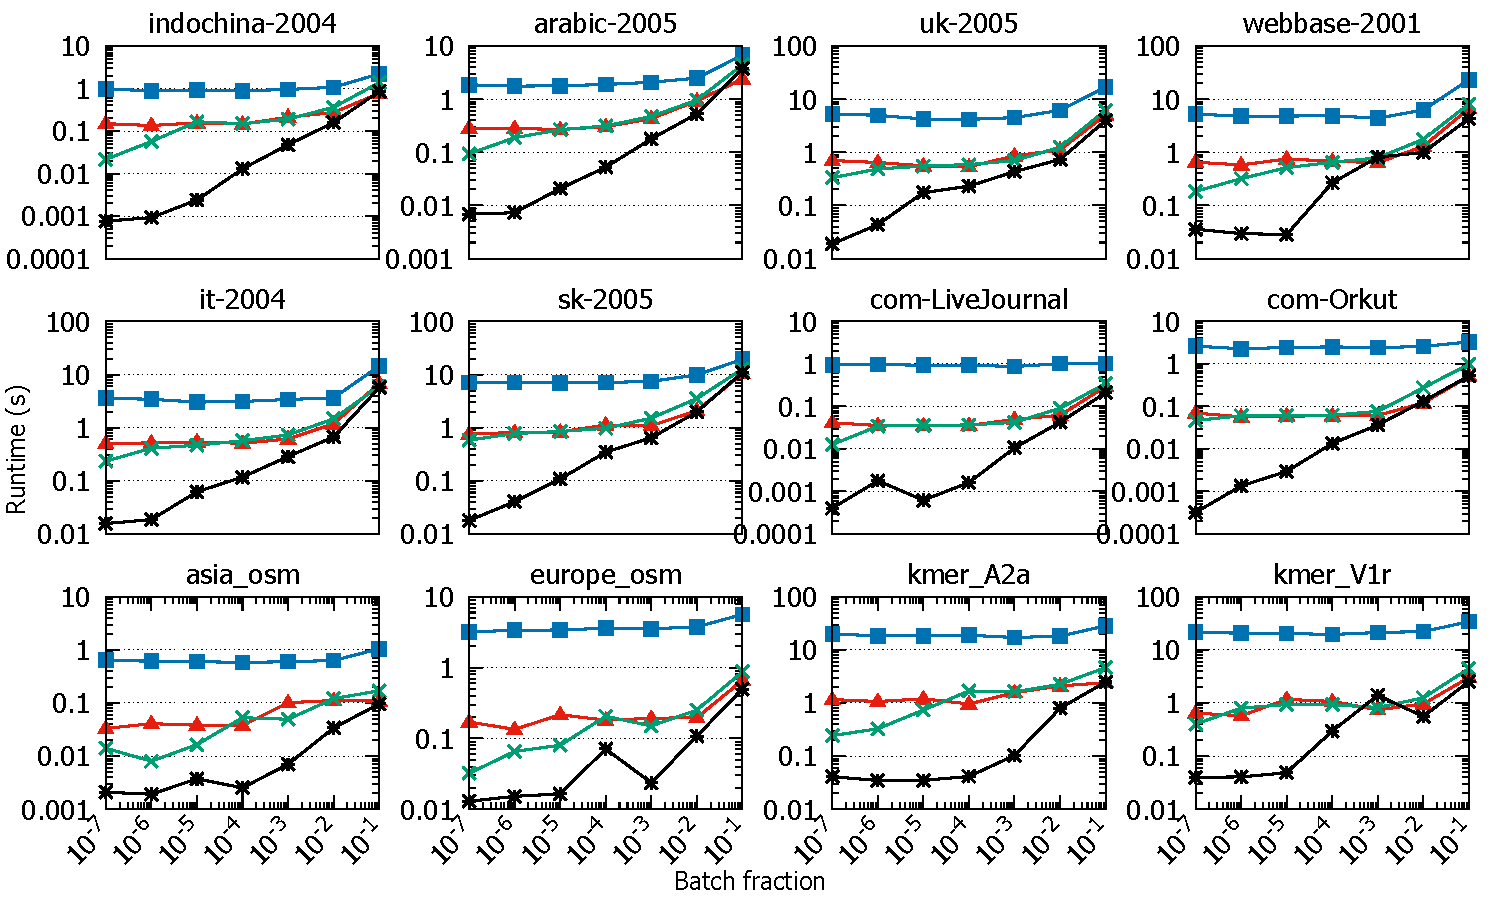
\includegraphics[width=0.58\linewidth]{out/8020-runtime-all.pdf}
  } \\[-1ex]
  \caption{Runtime (logarithmic scale) of GPU implementation for \textit{Static}, \textit{Naive-dynamic (ND)}, \textit{Dynamic Traversal (DT)}, \textit{Dynamic Frontier (DF)}, and \textit{Dynamic Frontier with Pruning (DF-P)} PageRank on large (static) graphs with generated random batch updates. Batch updates range in size from $10^{-7}|E|$ to $0.1|E|$ in multiples of $10$. These updates consist of $80\%$ edge insertions and $20\%$ edge deletions, mimicking realistic changes in a dynamic graph scenario. The right subfigure illustrates the runtime of each approach for individual graphs in the dataset, while the left subfigure presents overall runtimes (using geometric mean for consistent scaling across graphs). Additionally, the speedup of each approach relative to Static PageRank is labeled\ignore{on respective lines}.}
  \label{fig:8020-runtime}
\end{figure*}
